% !TeX root = ../../../book.tex

\subsection{等价类}

\subsubsection*{定义}

设 $R$ 为集合 $A$ 上的等价关系。如前所述,等价关系的三个性质——自反性、对称性和传递性——将集合 $A$ 划分为若干互不相交的子集。这些子集形成``封闭组织''或``簇'',其中任意元素均可代表整个子集,无需枚举所有成员。此类子集称为\emph{等价类},其形式化定义如下:

\begin{definition}
    设 $R$ 为集合 $A$ 上的等价关系,$x \in A$。$x$ 在关系 $R$ 下的\dotuline{等价类}记为 $[x]_R$,定义为所有与 $x$ 相关的元素组成的集合。即
    \[[x]_R = \{y \in A \mid (x,y) \in R\}\]
\end{definition}

\subsubsection*{引言与示例}

等价类的核心思想在于:通过关系 $R$ 可将集合 $A$ \textbf{划分}为若干标准子集。回顾第 \ref{ch:chapter03} 章定义 \ref{def:definition3.6.9} 对集合\textbf{划分}的说明(亦可参考定义 \ref{def:definition4.5.11} 的符号化表述)。划分的本质是:一组非空子集互不相交,且其并集构成原集合。

\begin{example}
    让我们回到本节一开始的例子。我们定义了实数集 $\mathbb{R}$ 上的关系 $R$,如下所示:
    \[\forall x, y \in \mathbb{R} \centerdot (x, y) \in \mathbb{R} \iff \lfloor x \rfloor = \lfloor y \rfloor\]
    现在,利用定义来思考一个特定的等价类。具体来说,我们来看
    \[[0]_R = \{y \in \mathbb{R} \mid (0, y) \in \mathbb{R}\} = \{\in \mathbb{R} \mid \lfloor 0 \rfloor = \lfloor y \rfloor\} = \{y \in \mathbb{R} \mid \lfloor y \rfloor = 0\} = \{y \in \mathbb{R} \mid 0 \le y < 1\}\]
    由上述定义可知,$[0]_R$ 即区间 $[0, 1)$,如下图所示:

    \begin{center}
        {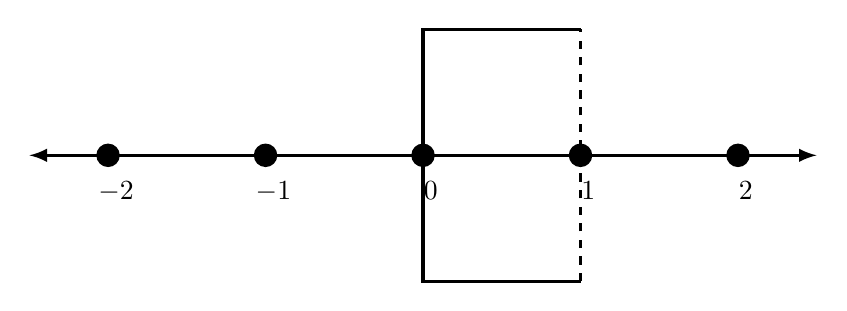
\begin{tikzpicture}[very thick,scale=2]
            \draw[latex-latex] (-2.5,0) -- (2.5,0); 
            \foreach \x in  {-2,-1,0,1,2}
            {
                \node at (\x, 0)[circle,fill,inner sep=3pt]{};
                \draw[shift={(\x+0.05,-0.1)}] node[below] {$\x$};
            }
            \draw[dashed] (1,-0.8) -- (1,0.8);
            \draw (1,0.8) -- (0,0.8) -- (0, -0.8) -- (1, -0.8);
        \end{tikzpicture}}
    \end{center}
    同理可得:
    \[[1]_R = \{y \in \mathbb{R} \mid (1, y) \in \mathbb{R}\} = \{y \in \mathbb{R} \mid 1 \le y < 2\}\]
    如下图所示:

    \begin{center}
        {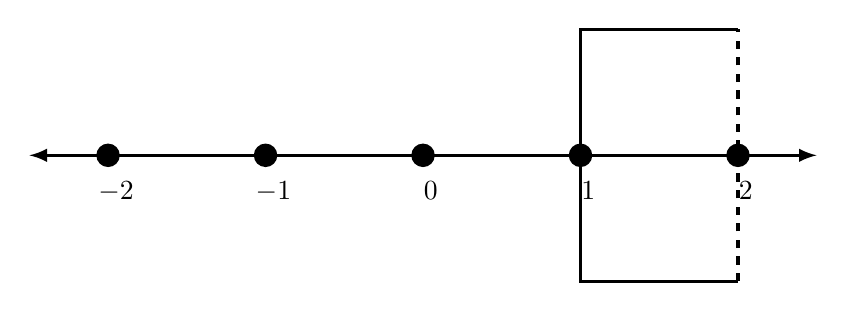
\begin{tikzpicture}[very thick,scale=2]
            \draw[latex-latex] (-2.5,0) -- (2.5,0); 
            \foreach \x in  {-2,-1,0,1,2}
            {
                \node at (\x, 0)[circle,fill,inner sep=3pt]{};
                \draw[shift={(\x+0.05,-0.1)}] node[below] {$\x$};
            }
            \draw[dashed] (2,-0.8) -- (2,0.8);
            \draw (2,0.8) -- (1,0.8) -- (1, -0.8) -- (2, -0.8);
        \end{tikzpicture}}
    \end{center}
\end{example}

注意到 $[0]_R$ 与 $[1]_R$ 互不相交(因为 $1 \notin [0]_R$ 而 $1 \in [1]_R$),且\textbf{每个实数必属于唯一}区间。例如:
\[\pi \in [3]_R, e \in [2]_R, -1.5 \in [-2]_R,\frac{1}{2} \in [0]_R\]
请注意,\emph{等价类}的定义并没有要求我们必须用某个特定元素来\emph{表示}该类。例如,我们也可以说
\[[0]_R = \Big[\frac{1}{2}\Big]_R\]
因为这两个集合是相等的,它们包含相同的元素。任何``向下取整''为 $0$ 的实数在 $R$ 下都与 $0$ 相关,因此在 $R$ 下也与 $\frac{1}{2}$ 相关,因为它们的向下取整都是 $0$。

建议通过此例深入理解划分的性质。后续我们将严格证明该性质的普适性!由于接下来的论证较为抽象,请结合具体实例思考:尝试在其他集合上定义等价关系,观察其等价类,理解其构成划分的必然性。

\subsubsection*{集合的等价类划分}

我们已探讨过等价类对集合的\emph{划分}思想,现在正式定义这个概念。首先给出定义,随后证明一个本质为``当且仅当''的定理。我们将证明其中一个方向,另一方向留作练习。

\begin{definition}
    设 $R$ 为集合 $A$ 上的等价关系,关系 $R$ 下等价类的集合记作 $A / R$,即 $A$ \dotuline{模 (modulo)} $R$。也就是说
    \[A / R = \{[x]_R \mid x \in A\}\]
    换种写法是
    \[A / R = \{X \subseteq A \mid \exists x \in A \centerdot X = [x]_R\}\]
\end{definition}

在证明核心结论前,先通过实例理解概念。每个例子需验证等价关系存在性,检验等价类,并思考模运算的作用。

\begin{example}
    再次考察实数集 $\mathbb{R}$ 上的关系 $R$,其定义为 $(x, y) \in R \iff \lfloor x \rfloor = \lfloor y \rfloor$。此前已说明它是等价关系,现在研究其等价类。

    根据定义,任何两个相关的元素都有相同的等价类。例如,$[0]_R = [0.5]_R = [0.999]_R$。同样地,$[3.5]_R = [3.75]_R, [-\pi]_R = [-4]_R$,但 $[\pi]_R \ne [4]_R$。每个实数 $x \in \mathbb{R}$ 都有一个对应的等价类 $[x]_R$,而模运算的思想是通过只考虑必要的等价类来简化 $R$ 的表示。由于 $[0]_R = [0.5]_R = [0.333]_R$ 等等,我们可以用一个集合 $[0]_R$ 来代表所有这些相同的集合。故有
    \[\mathbb{R} / R = \{\dots, [-2]_R, [-1]_R, [0]_R, [1]_R, [2]_R, \dots \}\]
    实际上,$\mathbb{R} / R$ 可与整数集 $\mathbb{Z}$ 建立对应。然而,我们通常写作 $\mathbb{R} / R ``='' \mathbb{Z}$ 是因为这种等式并不严谨。特别是,我们尚未形式化定义实数或整数,仅仅严格定义了自然数 $\mathbb{N}$。此处仅仅观察到等价类集与整数集存在对应关系,二者可以相互映射,但技术上并非\emph{相等}。

    不过没关系!本例重在说明 $\mathbb{R} / R$ 是等价类的集合。需注意,集合论中元素的顺序和重复无关紧要。如 $\{1, 3, 5, 3, 1\}$ 与 $\{1, 3, 5\}$ 在集合意义上是\emph{同一集合},因为它们含有\emph{相同元素}。同理,$\mathbb{R} / R$ 无需同时包含 $[0]_R$ 和 $[0.5]_R$(二者为同一对象),重复列出无意义。

    通常,我们会关注等价类的表征形式与定性描述,例如:$A/R$ 中类的数量、类的规模(是否等势?是否存在有限类与无限类?)、类元素的描述模式是否一致?

    本例中,$\mathbb{R} / R$ 的所有等价类结构相同。存在可数无限多个等价类(与 $\mathbb{Z}$ 一一对应),每个类均为无穷集且形如实数区间。具体而言,对任意 $z \in \mathbb{Z}$,有 $[z]_R = \{y \in \mathbb{R} \mid z \le y < z + 1\}$。故这些等价类具有\emph{相同结构}。
\end{example}

\begin{example}
    在所有人的集合 $S$ 上定义关系 $B$ 为 $(x, y) \in B \iff x \text{\ 和\ } y \text{\ 同月出生}$。那么 $(\text{欧拉}, \text{庞加莱}) \in B$ 且 $(\text{Paul Erdős}, \text{Emmy Noether}) \in B$。$B$ 是等价关系吗?是的,因为:每个人都与自己的出生月份相同(自反性);若 $x$ 与 $y$ 同月出生,则 $y$ 与 $x$ 必然同月出生(对称性);若 $x$ 与 $y$ 同月出生,且 $y$ 与 $z$ 同月出生,则 $x$ 与 $z$ 同月出生(传递性)。

    (注意:通常由``具有相同……''或``是同一……''定义的关系是等价关系。)

    在此关系下,等价类对应出生月份。每个等价类由同月出生的人组成。例如,Paul Erdős 和 Emmy Noether 均生于三月,故 $\text{Emmy Noether} \in [\text{Paul Erdős}]_B$。该等价类\emph{对应于}三月,但请注意,它是基于集合 $S$(全体人)中的特定元素定义的。

    若定义 $M$ 为所有三月出生者的集合,则 $M = [\text{Paul Erdős}]_B$。综上,按出生月份划分的集合 $S/B$ 包含 $12$ 个子集,每个子集对应一个月份,包含该月出生的所有人。
\end{example}

\begin{example}
    考虑所有有序实数对的集合 $\mathbb{R} \times \mathbb{R}$。在其上定义关系 $R$:
    \[\big((x, y),(u, v)\big) \in R \iff x = u\]
    也就是说,当平面上两点的横坐标相同时,它们在关系 $R$ 下相关。几何上,此关系只关心点所在与 $y$ 轴平行的垂线。由此可以直观理解 $R$ 是等价关系,严格证明只需按定义逐项验证即可。(请尝试证明!)

    该关系下的等价类很容易描述:所有在同一垂线上的点都属于同一个等价类,这些类可用垂线与横轴的交点索引。例如 $(1, 3) \in [(1, 0)]_R$,因为点 $(1, 3)$ 与 $(1, 0)$ 位于同一条垂线上。每个等价类均可表示为 $[(x, 0)]_R$,其中 $x \in \mathbb{R}$。
\end{example}

\begin{center}
    {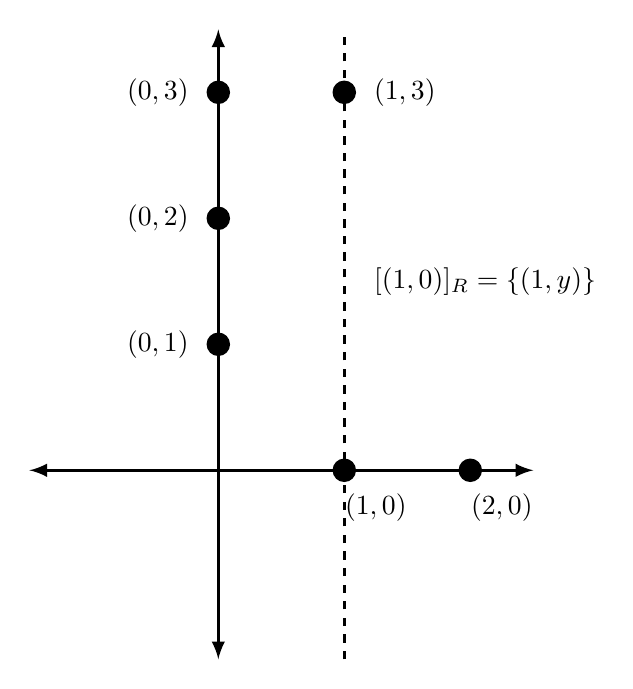
\begin{tikzpicture}[very thick,scale=1.6]
        \draw[latex-latex] (-1.5,0) -- (2.5,0); 
        \draw[latex-latex] (0,-1.5) -- (0,3.5); 
        \foreach \x in  {1,2}
        {
            \node at (\x, 0)[circle,fill,inner sep=3pt]{};
            \draw[shift={(\x+0.25,-0.1)}] node[below] {$(\x, 0)$};
        }
        \foreach \y in  {1,2,3}
        {
            \node at (0, \y)[circle,fill,inner sep=3pt]{};
            \draw[shift={(-0.15, \y)}] node[left] {$(0, \y)$};
        }
        \draw[dashed] (1,-1.5) -- (1,3.5);
        \node at (1, 3)[circle,fill,inner sep=3pt]{};
        \draw[shift={(1.15, 3)}] node[right] {$(1, 3)$};
        \draw[shift={(1.15, 1.5)}] node[right] {$[(1,0)]_R = \{(1, y)\}$};
    \end{tikzpicture}}
\end{center}

因此,在某种意义上,等价类的集合 $(\mathbb{R} \times \mathbb{R})/R$ 与实数轴 $\mathbb{R}$ ``等同''!通过忽略第纵坐标,我们可以将平面上的所有点投影到横轴上。从数学上讲,有一种更精确的方式表达这一观点,但这里不作正式讨论。简而言之,$\mathbb{R} \times \mathbb{R}$ 上的这一关系所生成的等价类对应于 $\mathbb{R}$,这带来了一些有趣的现象。

下面给出 $\mathbb{R} \times \mathbb{R}$ 上的另一个关系。定义 $S$ 为
\[\big((x, y),(u, v)\big) \in S \iff \sqrt{x^2+y^2} = \sqrt{u^2+v^2}\]
回顾基本几何与代数知识,不难发现 $\sqrt{x^2 + y^2}$ 表示点 $(x, y)$ 到原点 $(0, 0)$ 的距离。(在数学中,这类函数被称为\emph{度量 (metric)}。)因此,该关系表明,当两点到原点的距离相等时,它们是等价的。直观上,这解释了 $S$ 是等价关系,且等价类是以原点为中心的圆。于是,我们可以用这些圆的一个显著特征——它们的\emph{半径} $r \ge 0$,来描述集合 $(\mathbb{R} \times \mathbb{R})/S$ 的元素。因此,$S$ 下的等价类集合与非负实数集``等同''!

\begin{center}
    {\begin{tikzpicture}[very thick,scale=2]
        \draw[latex-latex] (-3,0) -- (3,0); 
        \draw[latex-latex] (0,-3) -- (0,3); 
        \foreach \x in  {-2,-1,0,1,2}
        {
            \node at (\x, 0)[circle,fill,inner sep=3pt]{};
            \node at (0, \x)[circle,fill,inner sep=3pt]{};
        }
        \draw[dashed] (0,0) circle (1);
        \draw[dashed] (0,0) circle (2);
        \draw[shift={(0.8, -0.7)}] node[right] {$[(1,0)]_S$};
        \draw[shift={(0.8, -0.9)}] node[right] {$r=1$};
        \draw[shift={(1.7, 1.5)}] node[right] {$[(2,0)]_S$};
        \draw[shift={(1.7, 1.3)}] node[right] {$r=2$};
    \end{tikzpicture}}
\end{center}

这听起来有点奇怪。我们从一个二维集合出发,关联点对并划分出等价类,最终却得到一个一维集合。(注意:我们尚未正式定义\emph{维度 (dimension)},但读者应该能够理解其含义。)回顾上文在 $\mathbb{R}^2$ 上定义的关系 $R$。如果我们将该关系限制在 $\mathbb{R}^2$ 的``右半部分'',即所有横坐标非负的点集上,那么等价类集合也与非负实数集``等同''。在何种意义上,此集合与 $(\mathbb{R} \times \mathbb{R})/S$ ``等同''?这个问题是否合理?我们又该如何\emph{证明}这一结论?这些都是值得思考的有趣问题!

不必过分纠结这些概念与问题。关键在于:等价类的集合构成了原集合的一个\textbf{划分}。

现在我们已经考察了若干例子,接下来我们将陈述(并证明!)等价关系的一些重要结论。核心在于,这些定理印证了我们反复强调的观点:等价关系将集合划分成相应的等价类。然而,有趣的是,我们还有一个逆向结论:给定任意划分,均可定义一个对应的等价关系!

\begin{theorem}\label{theorem6.4.10}
    设 $R$ 为集合 $A$ 上的等价关系。则 $A/R$ 中的集合构成 $A$ 的划分,即这些集合非空、互不相交,且其并集为 $A$。
\end{theorem}

\begin{proof}
    见习题 \ref{exc:exercises6.7.13}
\end{proof}

我们将在本章末尾的习题 \ref{exc:exercises6.7.13} 中引导你完成这一证明。此前讨论的例子有助于你直观理解该定理的正确性,而通过详细的证明推导,你将对其数学严谨性获得扎实的理解。

\subsubsection*{划分产生等价关系}

现在,我们考察一个类似但重要的结论,它实质上是前一个定理的逆命题。为了更好地理解这一定理,我们先分析一个例子,该例子也将提供定理证明的框架。

\begin{example}
    考虑集合 $S=[6]$。定义集合
    \[\mathcal{F} = \big\{ \{1, 4\}, \{2, 3, 5\} , \{6\} \big\}\]
    注意,$\mathcal{F}$ 构成 $S$ 的一个划分,因为这些集合是非空、互不相交,且并集为 $S$。是否存在等价关系 $R$ 使得 $S/R$ 恰好是这些集合?答案是肯定的!尽管难以用类似``$(x, y) \in R \iff x$ 与 $y$ 具有某种共同属性''这种优雅的形式定义,但可以利用划分本身构造关系。具体来说,划分集合就是等价类。划分本身建立了等价类的结构,我们只需通过 $(x, y) \in R \iff x \text{\ 与\ } y \text{\ 属于同一个划分集合}$ 来定义等价关系 $R$。

    本例中,设 $S_1 = \{1, 4\}, S_2 = \{2, 3, 5\}, S_3 = \{6\}$,则 $R$ 可以定义为
    \[(x, y) \in R \iff \exists i \in [3] \centerdot (x \in S_i \land y \in S_i)\]

    请思考为什么这种方法有效。它为何构成等价关系?其等价类是什么?
\end{example}

接下来正式陈述并证明该定理。

\begin{theorem}\label{theorem6.4.12}
    设 $S$ 为集合,$\mathcal{F}$ 为集合 $S$ 的划分。则存在等价关系 $R$ 使得 $S/R=\mathcal{F}$。
\end{theorem}

正如我们之前提到的,此结论的核心在于:划分的子集恰好可视为待定义的等价类。只需证明关系``$x$ 与 $y$ 相关当且仅当$x$ 和 $y$ 属于同一划分子集''是一个等价关系。这并不困难,建议在阅读证明前尝试自行推导!

\begin{proof}
    设 $\mathcal{F}$ 为集合 $S$ 的划分。这意味着存在索引集 $I$ 使得
    \[\mathcal{F} = {S_i \mid i \in I}\]
    其中集合 $S_i$ 满足 $S_i \subseteq S$ 且 $S_i \ne \varnothing$,并且
    \[\bigcup_{i \in I} S_i = S \quad \text{且} \quad \forall i, j \in I \centerdot i \ne j \implies S_i \cap S_j = \varnothing\]
    定义 $S$ 上的关系 $R$ 为
    \[(x, y) \in R \iff \exists i \in I \centerdot (x \in S_i \land y \in S_i)\]
    我们要证明 $R$ 为等价关系。

    \begin{itemize}
        \item \textbf{自反性}:设 $x \in S$ 为任意固定元素。由于 $S_i$ 覆盖 $S$,因此 $\exists i \in I \centerdot x \in S_i$。给定这样的 $i$,则必有 $x \in S_i$ 且 $x \in S_i$,因此 $(x,x) \in R$。故 $R$ 具有自反性。
        
        \item \textbf{对称性}:设 $x, y \in S$ 为任意固定元素。假设 $(x, y) \in R$,这意味着 $\exists i \in I \centerdot (x \in S_i \land y \in S_i)$。给定这样的 $i$,则必有 $y \in S_i \land x \in S_i$,因此 $(y,x) \in R$。故 $R$ 具有对称性。
        
        \item \textbf{传递性}:设 $x, y, z \in S$ 为任意固定元素。假设 $(x, y) \in R$ 且 $(y, z) \in R$,这意味着 $\exists i \in I \centerdot (x \in S_i \land y \in S_i)$ 且 $\exists j \in I \centerdot (y \in S_j \land z \in S_j)$。给定这样的 $i, j$,注意 $y \in S_i \land y \in S_j$,而对于任意不同的 $i,j, S_i \cap S_j = \varnothing$,因此 $i=j$(否则会出现 $y \in \varnothing$,而这是不可能的!)由于 $x \in S_i, y \in S_i, z \in S_i$,因此 $(x,z) \in R$。故 $R$ 具有传递性。
    \end{itemize}
    综上,$R$ 是一个等价关系!

    $S/R$ 的等价类写做 $[x]_R$,其中 $x \in S$。因为 $\mathcal{F}$ 是 $A$ 的划分,对于任意 $x \in S$,存在 $i$ 使得 $x \in S_i$。因此所有等价类均属于 $\mathcal{F}$。

    类似地,对于任意非空集合 $S_i \ne \varnothing$,都有 $\exists x \in S_i$,因此存在对应的等价类 $S_i=[x]_R$。故每个等价类都是形如 $S_i$ 的集合,反之亦然。
\end{proof}

这表明,任意划分都唯一对应一个等价关系及其等价类!
